\section[Thermodynamic consistency and closure limits of radiatively cooled X-point collapse]{\raggedright Thermodynamic consistency and closure limits of radiatively
cooled X-point
collapse}\label{thermodynamic-consistency-and-closure-limits-of-radiatively-cooled-x-point-collapse}

\textbf{Taylor Kalin}

Independent researcher; \url{https://taylorkalin.com}

ORCID: 0009-0003-9000-9315; correspondence:
\href{mailto:teylersf@gmail.com}{\nolinkurl{teylersf@gmail.com}}

Version 1.0.0; 29 October 2026

\subsection{Abstract}\label{abstract}

We examine the thermodynamic reduction in Chowdhry and Loureiro's model
of current-sheet formation under radiative cooling, using its journal
and arXiv editions. The displayed pressure formula does not solve the
stated energy equation. Direct integration gives a Bernoulli solution
whose initial cooling rate is nonzero, whereas the published
bremsstrahlung form has zero initial cooling rate for every finite
spatial integration coefficient. Correcting this formula generally
destroys the exact parabolic-pressure affine closure. On the common
positive-pressure branch, the corrected scalar evolution preserves
pressure ordering; in the published final ordinary differential
equations, outflow deceleration while the inflow scale is shorter than
the outflow scale requires negative central total pressure. Separately,
a cumulative cooling integral cannot be replaced by its vanishing
endpoint tail. At fixed finite coefficients and finite positive outflow
scale, that integral makes the printed cooling-to-magnetic force ratio
tend to zero, contradicting the proposed strict cooling-dominated
endpoint balance under those hypotheses. We retain the algebra of the
modified steady Sweet-Parker branch and state its parameter-domain and
stability limitations. Direct scalar integrations and separate
high-precision checks support these bounded conclusions. They do not
reconstruct the original numerical trajectories or rule out physical
radiative contraction in a different model.

\subsection{1. Target and scope}\label{target-and-scope}

Radiative cooling can change the pressure and compression of
reconnecting layers. Chowdhry and Loureiro {[}1,2{]} propose an affine
X-point-collapse model and a separate modification of a radiatively
cooled Sweet-Parker layer. Their abstract connects strong cooling to
accelerated inflow collapse and arrested or reversed outflow elongation.
The pressure reduction is therefore central to the proposed dynamical
explanation, rather than a peripheral normalization choice.

We examine the 26-page journal version of record, \emph{Journal of
Plasma Physics} \textbf{91}(6), E148 (2025), DOI
10.1017/S0022377825100949 {[}1{]}, and the supplied 24-page
arXiv:2508.13081v1 {[}2{]}. The supplied preprint is byte-identical to
the official versioned PDF. Both editions have been read completely. The
final article corrects the preprint's missing equality in Eq. (2.14),
updates the flow-rate symbols in Eq. (3.1), and adds cooling-law,
Newtonian-MHD and relativistic-applicability qualifications. Those
improvements are credited. The pressure construction, principal collapse
balances and steady-layer expressions addressed here remain in the final
edition. Locators below refer to {[}1{]} unless stated otherwise.

The main question is internal consistency: do the displayed reductions
satisfy the energy equation and their own positivity and asymptotic
assumptions? We derive the pressure evolution first, then examine its
spatial implications. Separate checks preserve the steady-layer algebra
instead of treating every conclusion as invalid. No original numerical
analysis program or complete set of execution inputs was obtained from
the inspected source archive. The original curves are not reproduced
here.

\subsection{2. The pressure initial-value
problem}\label{the-pressure-initial-value-problem}

Let \(J(t)=\xi(t)\eta(t)>0\) be the affine Jacobian, with the source's
normalization \(J(0)=1\), and \(\rho_L=\rho_0/J\). We use \(\bar C\) for
the positive coefficient already defined by the source's Eq. (2.22),
including its conversion factors. Equation (2.23) is

\[
\frac{d}{dt}\ln\left(\frac{P_L}{\rho_L^\gamma}\right)
=-\bar C\rho_L^{a-b}P_L^{b-1}. \tag{1}
\]

The derivative follows a fixed fluid label. Define

\[
Y=P_LJ^\gamma,\quad q=b(1-\gamma)+\gamma-a,\quad
\kappa=\bar C\rho_0^{a-b},\quad I(t)=\int_0^t J(t')^q\,dt'.
\]

Then Eq. (1) gives \(\dot Y=-\kappa J^qY^b\), with \(Y(0)=P_0\). On the
positive branch its unique solution is

\[
P_L=J^{-\gamma}
\left[P_0^{1-b}-(1-b)\kappa I(t)\right]^{1/(1-b)},
\qquad b\ne1, \tag{2}
\]

and

\[
P_L=J^{-\gamma}P_0\exp[-\kappa I(t)],\qquad b=1. \tag{3}
\]

For \(b<1\), Eq. (2) is used only while its bracket is positive.
Continuing a squared bremsstrahlung expression beyond its zero would
reverse the sign of the square root used in the derivation and cease to
solve the same positive-pressure equation. These formulas require no
special value of the initial pressure and no choice of an additional
spatial integration function.

In contrast, after choosing \(C_2=P_0\), the source's Eqs. (2.24)-(2.27)
and (A5)-(A6) have the functional form

\[
Y_{\rm pub}=P_0\left[1-\widetilde C I(t)^{1/(1-b)}\right]. \tag{4}
\]

This expression puts the initial pressure outside the nonlinear power.
It is not Eq. (2). The source also asserts that an independent spatial
\(C_2\) remains unconstrained after specifying the initial condition. A
first-order scalar initial-value problem on \(P_L>0\) has no such
freedom. In Appendix A, the equality between \(d\ln F/dt\) and
\(F^{-b}\dot F\) in Eq. (A4) already changes the left-hand side; adding
homogeneous and particular solutions does not repair a nonlinear
equation by superposition.

The bremsstrahlung case gives a normalization-independent
counterexample. With \(b=1/2\), Eq. (2) requires

\[
Y=\left(\sqrt{P_0}-\frac{\kappa I}{2}\right)^2,
\qquad \dot Y(0)=-\kappa\sqrt{P_0}\ne0. \tag{5}
\]

Every finite coefficient multiplying \(I^2\) in Eq. (4) instead gives
\(\dot Y_{\rm pub}(0)=0\) for regular \(J(0)>0\). Changing that finite
coefficient cannot recover the missing derivative. For the elementary
prescribed history \(J=1\), \(P_0=\kappa=1\), the correct pressure is
\((1-t/2)^2\) until \(t=2\); a printed-form example with
\(\widetilde C=1/4\) is \(1-t^2/4\). At \(t=1\) these give \(1/4\) and
\(3/4\). The numerical coefficient in this illustration is declared, not
inferred from an original plotted run.

\begin{minipage}{\linewidth}
\pandocbounded{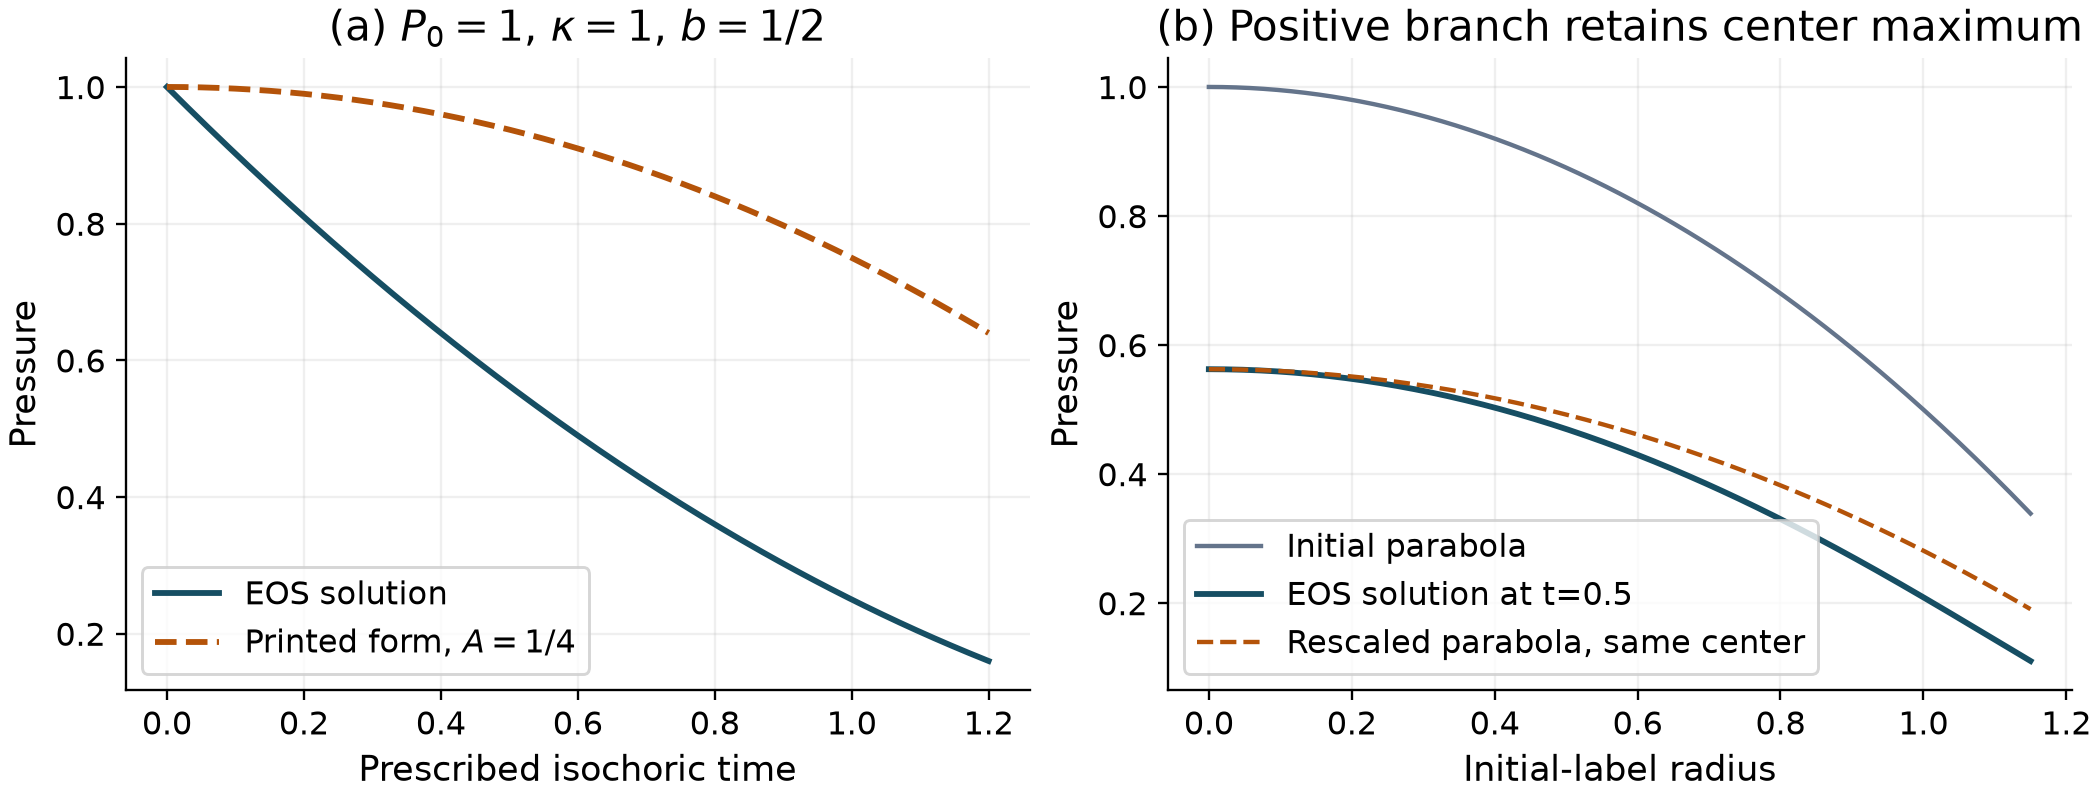
\includegraphics[keepaspectratio]{images/pressure-and-profile.png}}

Figure 1. Left: the isochoric bremsstrahlung solution has a nonzero
initial cooling slope; the printed functional form does not. Right: at
\(t=0.5\), an initially parabolic profile remains centrally maximal but
is not a common rescaling of that parabola. The dashed comparison is
matched at the center.
\end{minipage}

The discrepancy is not universal across all exponents. At \(b=0\), a
specifically calibrated additive coefficient can reproduce Eq. (2); it
is not arbitrary. At \(b=1\), the exponential solution must be treated
separately. These controls help distinguish the nonlinear integration
error from a blanket rejection of every cooling law.

\subsection{3. Spatial closure and the pressure
sign}\label{spatial-closure-and-the-pressure-sign}

The source chooses spatially uniform initial density and
\(P_0=P_{0,X}[1-(x_0^2+y_0^2)/2]\), then assumes a spatially uniform
\(J(t)\). For fixed common \(J\), differentiating the repaired solution
with respect to its positive initial value gives

\[
\frac{\partial P_L}{\partial P_0}
=J^{-\gamma}\left(\frac{Y}{P_0}\right)^b>0. \tag{6}
\]

Thus pressure ordering is preserved while both compared labels remain on
the positive branch. The initially higher central pressure cannot fall
below a lower surrounding pressure in this scalar, uniform-density
affine construction. Different fractional cooling rates do not by
themselves reverse the ordering. Once a label reaches the boundary of
the assumed cooling law, this comparison makes no assertion about
additional physics beyond it.

For \(b=1/2\), the factor in Eq. (6) is
\(J^{-\gamma}[1-\kappa I/(2\sqrt{P_0})]\). It depends on position
through \(P_0\). Multiplying the initial parabolic gradient by this
factor generally produces a non-affine force. Consequently, inserting
the correct pressure into momentum does not simply yield the source's
two scale-factor equations with a repaired time-only cooling factor.
Special cases such as \(b=0\), \(b=1\), uniform pressure or zero cooling
must be separated. A local Taylor expansion about the origin could
define an approximate closure, but that would be a new approximation
requiring its own validation, not the claimed exact global reduction.

There is also a direct positivity restriction inside the source's
\emph{printed} final Eq. (2.31). For bremsstrahlung, write
\(\theta=1-\widetilde C I^2\) and \(D=\xi^{-2}-\eta^{-2}\). Its outflow
acceleration becomes

\[
\ddot\eta=\xi\left[D+\frac{P_{0,X}\theta}{(\xi\eta)^\gamma}\right]. \tag{7}
\]

If \(0<\xi<\eta\), \(P_{0,X}>0\) and \(\theta\ge0\), every term on the
right is nonnegative and \(D>0\). Hence \(\ddot\eta>0\). Deceleration on
this branch requires \(\theta<0\), which is negative central \emph{total
thermal pressure} in Eq. (2.26). Negative pressure is necessary here,
not sufficient to outweigh the magnetic term. The pressure is not
defined as a freely adjustable perturbation; adding a constant
background changes an absolute-pressure nonlinear cooling law and
requires solving that law again.

This restriction matters for the interpretation in Section 3.3, which
invokes stronger nonuniform compression and a pressure maximum turning
into a minimum. The stated affine Jacobian and uniform initial density
instead give spatially uniform density at each time. Neither that
proposed density mechanism nor a positive-pressure central minimum
follows from the equations supplied. This does not prove that a
nonuniform-density plasma, a non-affine flow or a more complete
radiative-MHD model cannot contract along its outflow direction.

\subsection{4. Cumulative cooling and endpoint
balances}\label{cumulative-cooling-and-endpoint-balances}

A separate issue remains even if the published ODE is examined formally.
For \(a=2\), \(b=1/2\), \(\gamma=5/3\), Eq. (2.29) defines
\(I=\int_0^t(\xi\eta)^{-2/3}dt'\). Suppose \(\tau=t_c-t\),
\(\eta\to\eta_c>0\) and \(\xi\sim A\tau^\alpha\), with no earlier
singularity. For the proposed \(\alpha=2/3\) and \(\alpha=1\), the
endpoint is integrable:

\[
I_c-I(t)\sim
\frac{(A\eta_c)^{-2/3}}{1-2\alpha/3}\,
\tau^{1-2\alpha/3},\qquad 0<I_c<\infty. \tag{8}
\]

It is the tail \(I_c-I\), rather than the integral from the initial
time, that vanishes. The scaling substitution in Section 3.2 and
Appendix B drops this positive cumulative constant. It is leading order,
not a negligible integration term. In particular, the ratio of the
printed radiative-force magnitude to its inverse-square magnetic term is

\[
\mathcal D= P_{0,X}\widetilde C I(t)^2
\eta^{-\gamma}\xi^{2-\gamma}
\sim \mathrm{const.}\,\tau^{\alpha/3}\longrightarrow0. \tag{9}
\]

This limit uses fixed finite coefficients and a finite positive
\(\eta_c\). It contradicts a strict endpoint balance dominated by that
cooling term under those same hypotheses, including the proposed
intermediate equality in Eq. (3.13). A large coefficient can delay the
crossover greatly. The argument does not reject a finite-window
effective exponent near one, a joint infinite-cooling limit, or a branch
where \(\eta\) also vanishes. It also does not determine the physical
endpoint of the repaired, non-affine thermodynamic problem. Substituting
exactly \(\alpha=1\) into a second-derivative leading balance
additionally requires care because \(\alpha(\alpha-1)=0\).

\begin{minipage}{\linewidth}
\pandocbounded{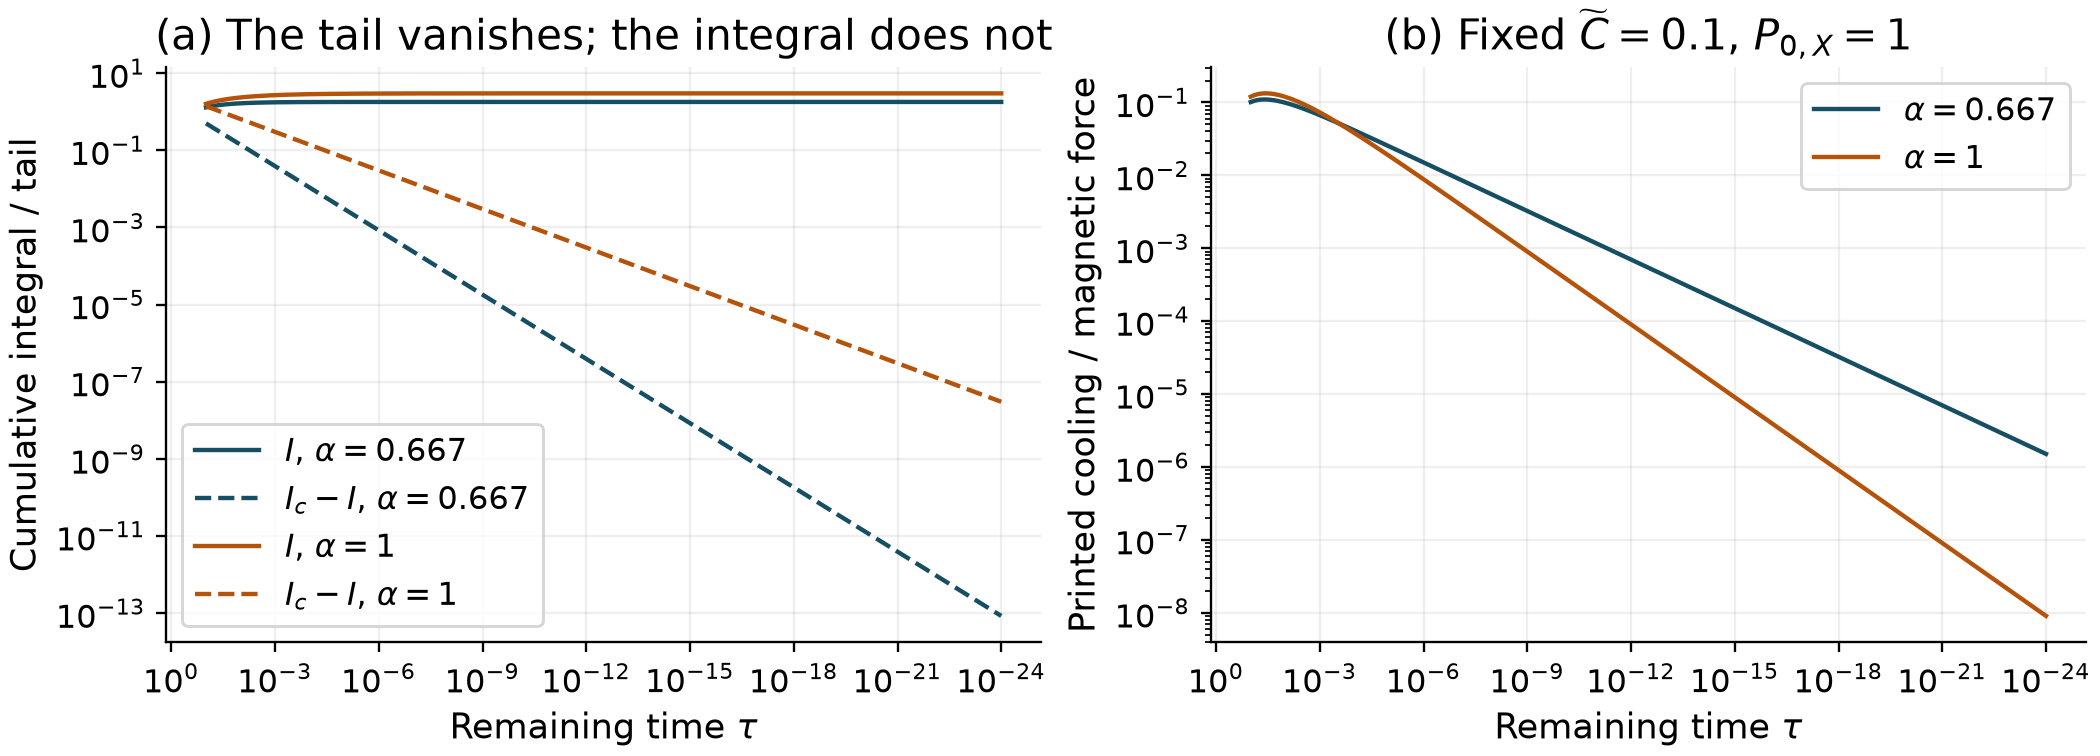
\includegraphics[keepaspectratio]{images/cumulative-integral.png}}

Figure 2. For \(t_c=1\), \(\eta=1\), \(\xi=\tau^\alpha\), the cumulative
limit is \(I_c=1/(1-2\alpha/3)\): \(1.8\) or \(3\). The force ratio uses
fixed \(P_{0,X}=1\) and \(\widetilde C=0.1\). The printed pressure
factor remains positive in both examples. The small remaining-time
values illustrate an analytic limit; they are not measured physical
collapse times.
\end{minipage}

The leading inverse-square scalar equation also fixes a coefficient:
\(\ddot\xi=-\eta_c/\xi^2\) requires \(A^3=9\eta_c/2\) for
\(\xi=A\tau^{2/3}\). Appendix B's Eq. (B14) instead prints
\(9\eta_c/4\), giving half the required acceleration. The missing factor
is visible between its kinetic-energy first integral and quadrature.
This is a discrepancy in the target's displayed calculation, not an
allegation about the classical literature it cites.

Retaining a generic finite net thermal coefficient has a further
consequence. Define
\(H_c=P_{0,X}\eta_c^{1-\gamma}(\widetilde C I_c^2-1)\). The frozen
leading scalar equation is
\(\ddot\xi=-\eta_c\xi^{-2}-H_c\xi^{-5/3}+\cdots\). When \(H_c\ne0\), its
first thermal correction is

\[
\xi=A\tau^{2/3}+D_1\tau^{8/9}+\cdots,
\qquad D_1=\frac{81}{44}H_cA^{-5/3}. \tag{10}
\]

This follows by linearizing the inverse-square force as well as
expanding the second derivative. A free scalar-energy correction of
order \(\tau^{4/3}\) is recovered in the zero-thermal-force control; it
is not generically the first thermal correction when \(H_c\ne0\). These
are local consistency expansions of reduced equations, not a global
existence theorem for the source initial data.

\subsection{5. Normalization and the steady
branch}\label{normalization-and-the-steady-branch}

Some local printed discrepancies can be identified without using the
pressure solution. Using the approximate right-hand side printed in Eq.
(2.33) and the outflow time in Eq. (2.34), with
\(D_0=\bar C\rho_0^{a-b}P_{0,X}^{b-1}\), their ratio is
\(R=D_0/\Gamma_{y,0}\). Equation (2.35) instead multiplies by
\(\Gamma_{y,0}\). A unit normalized initial rate masks the difference.
The literal pressure-over-radiated-power definition would give
\(D_0/[(\gamma-1)\Gamma_{y,0}]\); either clock retains division by the
outflow rate. Equation (2.36) also reverses \(1-b\) to \(b-1\) relative
to Eq. (2.27); bremsstrahlung's squared exponent masks that sign.
Neither discrepancy establishes which values an unavailable plotting
implementation used. These clock-convention factors are distinct from
the energy-equation failure.

The separate steady model deserves a positive control. Its continuity,
Ohm's-law, power and cooling/advection balances give Eqs. (4.7)-(4.16),
including \(A\approx1+\beta\), consistently within their displayed
approximations. Here \(A=\rho_X/\rho_{\rm in}\) denotes compression,
rather than the collapse amplitude, and \(\beta=\beta_{\rm in}\). We
retain these balances. With \(c=(\gamma-1)/\gamma^{3/2}\), the
bremsstrahlung branch is

\[
\lambda\equiv\frac{L}{L_{\rm sys}}
=\frac{c}{\mathcal R\beta(1+\beta)},\qquad
F\equiv\frac{v_{\rm in}/V_A}{S_{\rm sys}^{-1/2}}
=\left[\frac{\mathcal R\beta(1+\beta)^2}{c}\right]^{1/2}. \tag{11}
\]

Here \(\mathcal R\) is the source's system-scale cooling parameter, not
the collapse-time \(R\). The comparison is with the classical
incompressible Sweet-Parker scaling {[}4{]}. The source already neglects
order-one outflow factors; Eq. (11) uses its displayed conventions, not
an exact coefficient calibration.

Nevertheless, \(\mathcal R\gg1\) alone is not uniform in upstream beta.
A layer fitting the system requires \(\mathcal R>c/[\beta(1+\beta)]\).
Enhancement requires \(\mathcal R>c/[\beta(1+\beta)^2]\). At fixed
\(S_{\rm sys}\), increasing cooling indefinitely also leaves the thin,
slow-inflow branch:

\[
\frac{\delta}{L}=\left[\frac{\mathcal R\beta}{cS_{\rm sys}}\right]^{1/2},
\qquad
\frac{v_{\rm in}}{V_A}=\left[\frac{\mathcal R\beta(1+\beta)^2}
{cS_{\rm sys}}\right]^{1/2}. \tag{12}
\]

For \(\gamma=5/3\) and \(S_{\rm sys}=10^8\), three examples distinguish
a retained branch from extrapolations outside it:


\begin{minipage}{\linewidth}\small
\begin{tabular}{@{}
  >{\raggedleft\arraybackslash}p{(\linewidth - 8\tabcolsep) * \real{0.2000}}
  >{\raggedleft\arraybackslash}p{(\linewidth - 8\tabcolsep) * \real{0.2000}}
  >{\raggedleft\arraybackslash}p{(\linewidth - 8\tabcolsep) * \real{0.2000}}
  >{\raggedleft\arraybackslash}p{(\linewidth - 8\tabcolsep) * \real{0.2000}}
  >{\raggedright\arraybackslash}p{(\linewidth - 8\tabcolsep) * \real{0.2000}}@{}}
\toprule\noalign{}
\begin{minipage}[b]{\linewidth}\raggedleft
\(\beta\)
\end{minipage} & \begin{minipage}[b]{\linewidth}\raggedleft
\(\mathcal R\)
\end{minipage} & \begin{minipage}[b]{\linewidth}\raggedleft
\(L/L_{\rm sys}\)
\end{minipage} & \begin{minipage}[b]{\linewidth}\raggedleft
\(F\)
\end{minipage} & \begin{minipage}[b]{\linewidth}\raggedright
Interpretation
\end{minipage} \\
\midrule\noalign{}
\(1\) & \(100\) & \(0.001549\) & \(35.93\) & Fits, thin, sub-Alfvenic \\
\(10^{-6}\) & \(100\) & \(3098\) & \(0.01797\) & Layer exceeds system \\
\(1\) & \(10^{10}\) & \(1.549\times10^{-11}\) & \(3.593\times10^5\) &
Not thin or slow inflow \\
\bottomrule\noalign{}
\end{tabular}
\end{minipage}


The low-beta example is not an admissible counterexample to a branch
explicitly restricted to \(L<L_{\rm sys}\). It shows why that
restriction must accompany a conclusion based only on large
\(\mathcal R\). At fixed positive beta and suitable Lundquist number,
the source's shortened-layer enhancement remains possible.

\begin{minipage}{\linewidth}
\pandocbounded{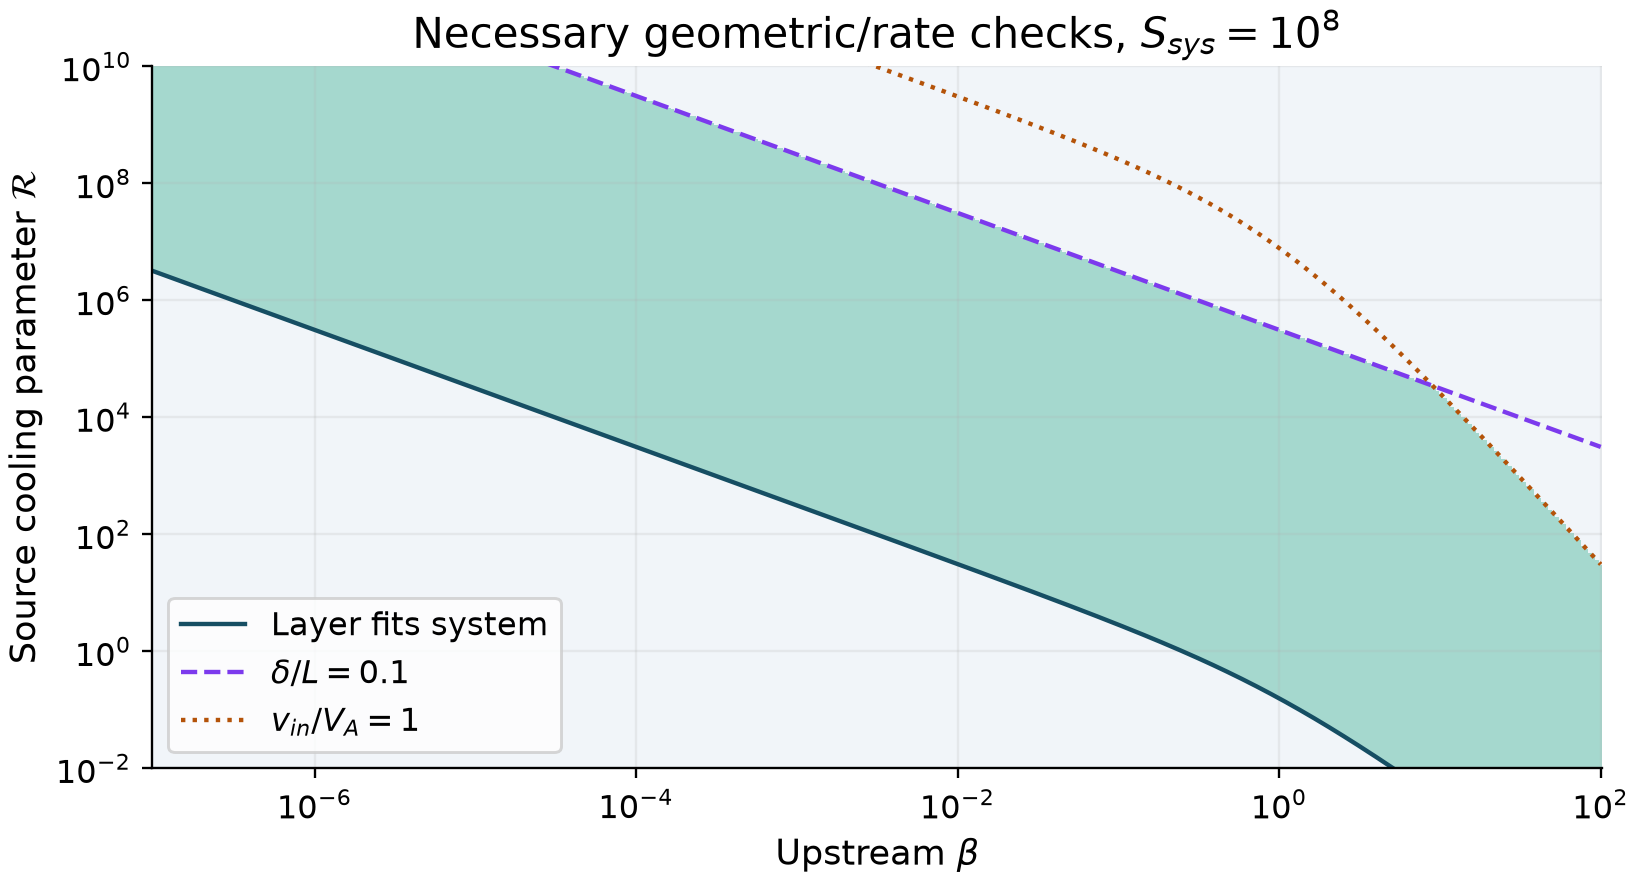
\includegraphics[keepaspectratio]{images/steady-branch-domain.png}}

Figure 3. Shading satisfies \(L<L_{\rm sys}\), \(\delta/L<0.1\) and
\(v_{\rm in}<V_A\) under the displayed conventions. The \(0.1\)
threshold is an illustrative thinness choice. No numerical threshold for
\(\mathcal R\gg1\), optical thinness, collisional validity or thermal
stability is imposed; the shading alone does not certify them.
\end{minipage}

Finally, an algebraic steady solution does not establish thermal
stability or evolutionary accessibility. Uzdensky and McKinney {[}3,
Section 4.1{]} explicitly distinguish these questions for their model
and derive a bremsstrahlung instability condition. Allowing length to
vary changes the possible branch, but the target supplies no dynamical
length-response law or perturbation spectrum proving its stability. We
do not transfer the earlier fixed-closure instability criterion
unchanged to this new branch, nor infer stability from the mere
existence of Eqs. (4.14)-(4.16).

\subsection{6. Verification, limitations and
conclusion}\label{verification-limitations-and-conclusion}

Three original figures and deterministic scalar examples accompany
independent verifiers {[}5{]}. The pressure verifier integrates the
original scalar pressure equation directly with DOP853, rather than
integrating its transformed solution. Independent 65-digit quadrature
then evaluates Eqs. (2)-(3). Eighty parameter/history reference
controls, within 318 scalar integrations, agree to a maximum relative
pressure difference \(9.76\times10^{-16}\) in the recorded environment.
Twenty groups of eleven ordered initial pressures retain ordering.
Spatial differences of separately integrated pressures agree with
high-precision derivatives to a maximum absolute difference
\(3.36\times10^{-10}\); the bremsstrahlung force coefficient varies
across labels while the \(b=0,1\) controls remain spatially constant.
All 4,096 seeded nonnegative-pressure outflow states, including one
zero-pressure control, satisfy Eq. (7)'s strict acceleration sign.

A separate 150-digit Decimal calculation compares 48- and 96-point
scalar quadratures, checks cumulative limits down to \(\tau=2^{-320}\),
and verifies the coefficient and reduced-equation subleading controls.
Another independent calculator checks nine cooling-clock examples, six
rational real-power sign cases, 24 parameter cases checking the
steady-state identities, and four branch-domain cases. The verifiers do
not import the plotting producer. Agreement is numerical and algebraic
evidence, not physical accuracy, independent human review or bitwise
reproducibility across arbitrary environments.

The source authors' five figures, unprovided numerical execution
parameters and original trajectories are not re-created. The pressure
examples impose volume histories solely to test the energy equation. No
full MHD/PIC calculation, repaired global affine evolution, physical
collapse time or empirical replacement for the source's critical cooling
threshold is claimed. Non-affine compression, density variation,
heating, conduction, resistivity and breakdown of a cooling law can
change the problem. A quoted numerical bremsstrahlung coefficient
remains under-specified in temperature/composition conventions and is
not promoted as a verified error. Minor presentation discrepancies are
recorded separately from the main findings.

The supported correction is substantive but bounded: the displayed
pressure solution fails its governing equation, and restoring it removes
the proposed exact global closure in the generic bremsstrahlung case.
Positive-pressure restrictions and the retained cumulative integral
further limit the stated flow-reversal and endpoint interpretations. The
separate steady-branch algebra survives, accompanied by its necessary
domain and unanswered stability questions.

\textbf{Code and data availability.} Original code, numerical outputs,
figure sources, source-edition hashes and portable independent verifiers
are archived as software version 1.0.0 {[}5{]},
\url{https://doi.org/10.5281/zenodo.23780790} , direct record
\url{https://zenodo.org/records/23780790} . The frozen computational
commit is \nolinkurl{8a4e64cc032cb0c57bb621b200903b0c0f0706c2} in
\url{https://github.com/Teylersf/radiative-cooling-current-sheet-audit}
. The anonymous archive download matches all 36 frozen files, and a
clean extraction reproduced all four programs without changing those
bytes. The DOI was independently verified as \nolinkurl{findable} in its
primary DataCite registry on 29 October 2026; a Crossref-only lookup
does not test this registration. Source PDFs are linked through their
official records and are not bundled as this author's work.

\textbf{Funding and disclosures.} Taylor Kalin self-funds this study. No
outside funding or competing interests have been reported. AI tools
assisted with source retrieval, derivation, code, adversarial checks and
drafting. These checks are not independent human peer review. The source
authors and institutions have not endorsed this work. Original code is
MIT licensed; original audit text and figures are CC BY 4.0. Attributed
third-party material retains its rights.

\clearpage
\begingroup\small\raggedright
\subsection{References}\label{references}

{[}1{]} S. Chowdhry and N. F. Loureiro, \emph{Current sheet formation
under radiative cooling}, Journal of Plasma Physics \textbf{91}(6), E148
(2025). \url{https://doi.org/10.1017/S0022377825100949} . Version of
record, published online 7 November 2025.

{[}2{]} S. Chowdhry and N. F. Loureiro, \emph{Current sheet formation
under radiative cooling}, arXiv:2508.13081v1 (18 August 2025).
\url{https://arxiv.org/abs/2508.13081v1} ;
\url{https://arxiv.org/pdf/2508.13081v1} . Earlier edition, inspected
separately from {[}1{]}.

{[}3{]} D. A. Uzdensky and J. C. McKinney, \emph{Magnetic reconnection
with radiative cooling. I. Optically thin regime}, Physics of Plasmas
\textbf{18}, 042105 (2011). \url{https://doi.org/10.1063/1.3571602} .
The accessible author preprint, \url{https://arxiv.org/abs/1007.0774v1}
(2010), Section 4.1, pp.19-21, explicitly separates stationary
existence, evolutionary accessibility and thermal stability.

{[}4{]} E. N. Parker, \emph{Sweet's mechanism for merging magnetic
fields in conducting fluids}, Journal of Geophysical Research
\textbf{62}(4), 509-520 (1957).
\url{https://doi.org/10.1029/JZ062i004p00509} .

{[}5{]} T. Kalin, \emph{Computational evidence for Thermodynamic
consistency and closure limits of radiatively cooled X-point collapse},
software version 1.0.0, Zenodo (2026).
\url{https://doi.org/10.5281/zenodo.23780790} ;
\url{https://zenodo.org/records/23780790} . Registered with DataCite:
\url{https://api.datacite.org/dois/10.5281/zenodo.23780790} .
Computational snapshot
\nolinkurl{8a4e64cc032cb0c57bb621b200903b0c0f0706c2}.

\endgroup
